\PassOptionsToPackage{table}{xcolor}
\documentclass[aspectratio=169,professionalfonts]{beamer}

\usepackage{fontspec}
\setsansfont{Arial}
\setmonofont{Consolas}[Scale=0.82]
\usepackage{booktabs,tabularx,array,graphicx,adjustbox}
\usepackage{xcolor}
\usepackage{colortbl}
\usepackage{amsmath}
\usepackage{hyperref}

\definecolor{navy}{HTML}{0F243E}
\definecolor{teal}{HTML}{1F7A8C}
\definecolor{orange}{HTML}{D56B11}
\definecolor{ink}{HTML}{16202A}
\definecolor{muted}{HTML}{52606D}
\definecolor{pale}{HTML}{EAF4F5}

\usetheme{default}
\setbeamertemplate{navigation symbols}{}
\setbeamertemplate{frametitle}{%
  \nointerlineskip
  \begin{beamercolorbox}[wd=\paperwidth,ht=0.88cm,dp=0.22cm,leftskip=0.55cm]{frametitle}
    \usebeamerfont{frametitle}\insertframetitle
  \end{beamercolorbox}}
\setbeamertemplate{footline}{%
  \hbox{\begin{beamercolorbox}[wd=\paperwidth,ht=2.5ex,dp=1.2ex,leftskip=0.5cm,rightskip=0.5cm]{author in head/foot}%
    \color{muted}\scriptsize NASA C-MAPSS FD001--FD004\hfill\insertframenumber/\inserttotalframenumber
  \end{beamercolorbox}}}
\setbeamercolor{normal text}{fg=ink,bg=white}
\setbeamercolor{frametitle}{fg=white,bg=navy}
\setbeamercolor{structure}{fg=teal}
\setbeamercolor{block title}{fg=white,bg=teal}
\setbeamercolor{block body}{fg=ink,bg=pale}
\setbeamercolor{alertblock title}{fg=white,bg=orange}
\setbeamercolor{alertblock body}{fg=ink,bg=orange!10}
\setbeamerfont{frametitle}{size=\Large,series=\bfseries}
\setbeamerfont{block title}{size=\normalsize,series=\bfseries}
\setbeamerfont{block body}{size=\normalsize}
\setbeamersize{text margin left=0.55cm,text margin right=0.55cm}
\setlength{\tabcolsep}{5pt}
\newcommand{\source}[1]{\vfill\hspace{0pt}\scriptsize\color{muted}Nguồn: \nolinkurl{#1}}
\newcommand{\metric}[2]{\textcolor{teal}{\textbf{#1}}\;#2}
\newcolumntype{L}[1]{>{\raggedright\arraybackslash}p{#1}}
\rowcolors{2}{pale}{white}
\arrayrulecolor{navy}

\title{Dự đoán RUL và kiểm tra chuyển miền}
\subtitle{NASA C-MAPSS FD001--FD004}
\author{Phan Nguyễn Mai Phương \quad | \quad MSHV 25002711}
\institute{Báo cáo cuối kỳ môn Phân tích dữ liệu lớn}
\date{Tháng 9 năm 2026}

\begin{document}

{\setbeamertemplate{background canvas}{\color{navy}\rule{\paperwidth}{\paperheight}}
\setbeamercolor{normal text}{fg=white,bg=navy}
\begin{frame}[plain]
  \vspace*{0.55cm}
  {\color{white}\fontsize{27}{31}\selectfont\bfseries Dự đoán tuổi thọ còn lại\\[0.12cm] và kiểm tra chuyển miền\par}
  \vspace{0.3cm}
  {\color{pale}\Large NASA C-MAPSS FD001--FD004\par}
  \vspace{0.55cm}
  {\color{white}\normalsize Báo cáo cuối kỳ môn Phân tích dữ liệu lớn\par}
  \vspace{0.25cm}
  {\color{white}\normalsize Phan Nguyễn Mai Phương \quad | \quad MSHV 25002711\par}
\end{frame}}

\begin{frame}{Bài toán nghiên cứu}
\begin{columns}[T,onlytextwidth]
\column{0.48\textwidth}
\textcolor{teal}{\Large\bfseries Đầu vào}

Chuỗi đo của 21 sensor theo từng cycle và từng engine.

\vspace{0.8cm}
\textcolor{teal}{\Large\bfseries Đầu ra}

Remaining Useful Life (RUL): số cycle còn lại trước failure.

\column{0.48\textwidth}
\begin{block}{Ví dụ tạo nhãn train}
Nếu engine kết thúc ở cycle 200 thì tại cycle 170:
\[
\mathrm{RUL}=200-170=30\ \text{cycles}.
\]
\end{block}

Test bị cắt trước failure; nhãn test chỉ dùng sau khi ghi dự đoán cuối.
\end{columns}
\source{report/sections/problem-data.tex; data/CONTRACTS.md}
\end{frame}

\begin{frame}{Dữ liệu C-MAPSS và ranh giới nhãn}
\begin{table}
\centering\small
\begin{tabular}{lrrl}
\toprule
Subset & Train engines & Test engines & Điều kiện / fault mode\\
\midrule
FD001 & 100 & 100 & 1 condition / 1 fault mode\\
FD002 & 260 & 259 & 6 conditions / 1 fault mode\\
FD003 & 100 & 100 & 1 condition / 2 fault modes\\
FD004 & 249 & 248 & 6 conditions / 2 fault modes\\
\bottomrule
\end{tabular}
\end{table}

\vspace{0.25cm}
Protocol chính dùng FD001: 20.631 train observations và 13.096 test observations.

\begin{alertblock}{Data leakage boundary}
Test labels của từng subset chỉ được đọc sau khi final predictions đã được ghi.
\end{alertblock}
\source{data/raw/DATA_SOURCE.md; NASA C-MAPSS metadata}
\end{frame}

\begin{frame}{Quy trình xử lý dữ liệu}
\centering
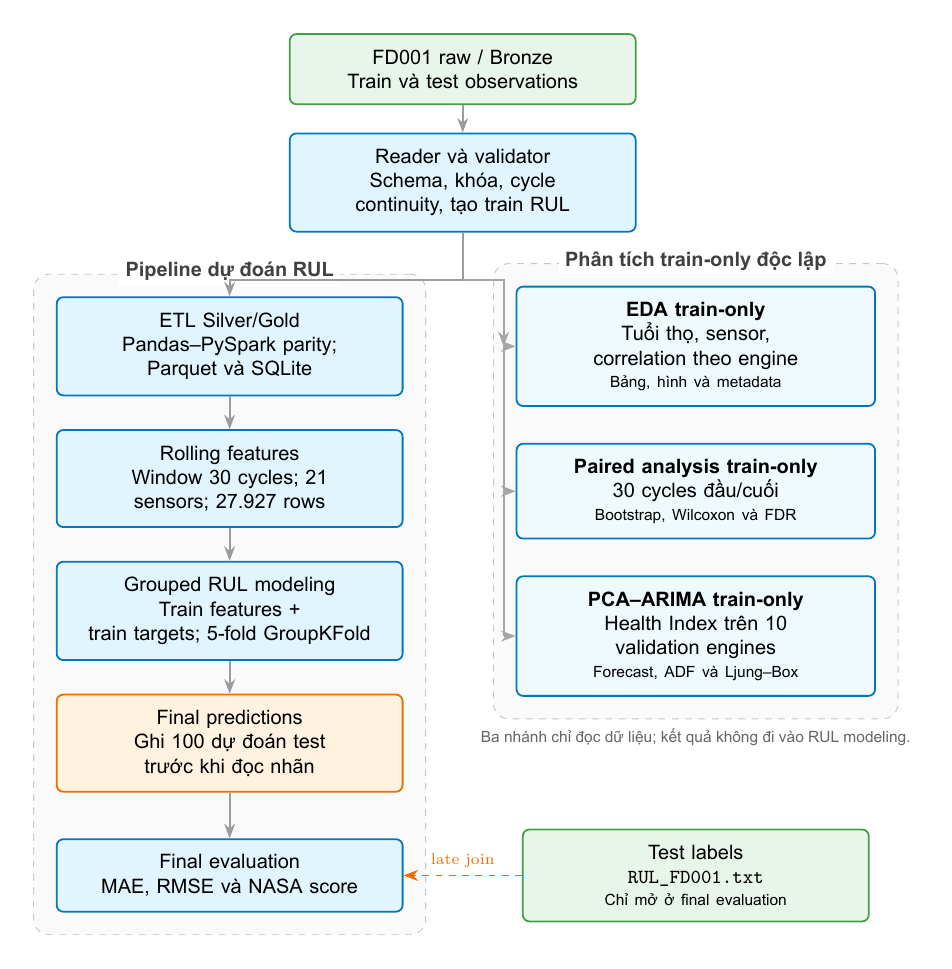
\includegraphics[width=0.96\textwidth,height=0.63\textheight,keepaspectratio]{../assets/diagrams/fd001-pipeline.png}

\vspace{0.15cm}
\textcolor{navy}{\bfseries Raw validation $\rightarrow$ Silver/Gold ETL $\rightarrow$ rolling features $\rightarrow$ GroupKFold $\rightarrow$ final evaluation}
\source{assets/diagrams/fd001-pipeline.png; outputs/modeling/tables/evaluation_protocol.csv}
\end{frame}

\begin{frame}{Sensor thay đổi theo vòng đời}
\begin{columns}[T,onlytextwidth]
\column{0.52\textwidth}
\textcolor{teal}{\Large\bfseries Protocol}

So sánh mean của 30 cycles đầu và 30 cycles cuối trong cùng một train engine.

\vspace{0.35cm}
Bootstrap theo engine, Wilcoxon signed-rank và Benjamini--Hochberg cho 21 sensor.

\column{0.43\textwidth}
\begin{block}{Kết quả}
15 sensor bác bỏ giả thuyết không sau hiệu chỉnh BH.
\end{block}

Kết quả mô tả thay đổi đầu/cuối vòng đời. Kết quả chưa phải bằng chứng nhân quả
hoặc feature selection cho engine mới.
\end{columns}
\source{outputs/statistics/tables/sensor_inference.csv}
\end{frame}

\begin{frame}{Từ chuỗi sensor đến đặc trưng}
\begin{block}{Trailing window 30 cycles}
Tại cycle 170, window dùng cycles 141--170 của cùng engine; không dùng quan sát tương lai.
\end{block}

\begin{table}
\centering\small
\begin{tabular}{ll}
\toprule
Đặc trưng & Vai trò\\
\midrule
Giá trị cuối & Trạng thái tại cycle hiện tại\\
Mean, sample standard deviation & Mức và biến thiên trong window\\
Min, max, linear slope & Biên và xu hướng tăng/giảm\\
\bottomrule
\end{tabular}
\end{table}

\centering
\textcolor{teal}{\Large\bfseries 21 sensor $\times$ 6 phép tóm tắt = 126 feature columns}

\source{outputs/features/run_info.json; report/sections/methodology.tex}
\end{frame}

\begin{frame}{Đánh giá theo engine}
\begin{table}
\centering\small
\begin{tabular}{lll}
\toprule
Giai đoạn & Dữ liệu & Mục đích\\
\midrule
5-fold GroupKFold & 100 train engines & Chọn model bằng mean engine MAE\\
Refit & Toàn bộ train & Tạo model cuối\\
Final test & 100 test engines & Một dự đoán tại cycle cuối mỗi engine\\
\bottomrule
\end{tabular}
\end{table}

\begin{alertblock}{Vì sao chia theo engine?}
Các window trong cùng engine có phụ thuộc thời gian. Chia ngẫu nhiên theo row
có thể đưa window gần nhau vào cả train và validation, làm metric lạc quan.
\end{alertblock}
\source{outputs/modeling/tables/evaluation_protocol.csv}
\end{frame}

\begin{frame}{Lựa chọn model}
\begin{table}
\centering\small
\begin{tabular}{lrl}
\toprule
Model & Mean engine MAE & Vai trò\\
\midrule
Median baseline & 46,9543 & Mốc dự đoán hằng\\
Ridge & 23,9922 & Quan hệ tuyến tính\\
HistGradientBoosting & 20,2143 & Được chọn\\
\bottomrule
\end{tabular}
\end{table}

HistGradientBoosting được chọn vì có MAE thấp nhất trong ba ứng viên và trong
protocol cross-validation đã định trước.
\source{outputs/modeling/tables/model_metrics.csv}
\end{frame}

\begin{frame}{Kết quả chính trên FD001}
\begin{columns}[T,onlytextwidth]
\column{0.56\textwidth}
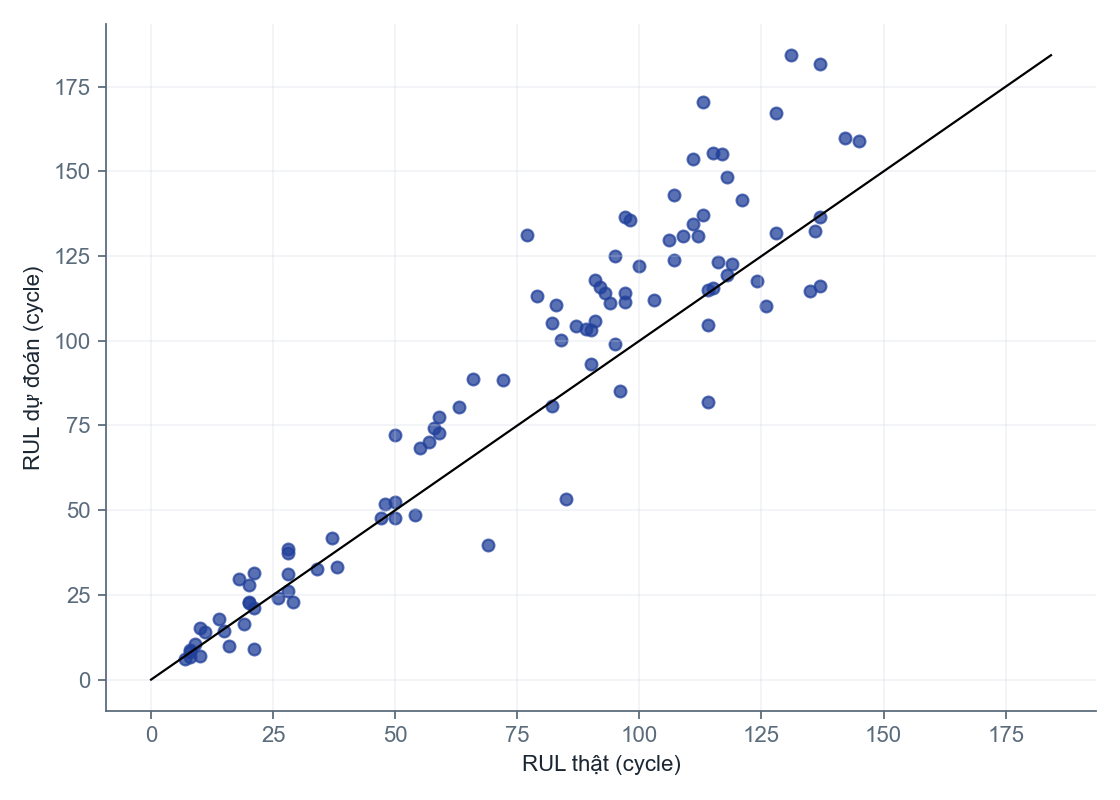
\includegraphics[width=\textwidth]{../outputs/modeling/figures/final_true_vs_predicted.png}
\column{0.40\textwidth}
\metric{MAE}{15,3490 cycles}

\vspace{0.25cm}
\metric{RMSE}{20,5413 cycles}

\vspace{0.25cm}
\metric{NASA score}{1.513,2577}

\vspace{0.25cm}
CI 95\% của MAE: [12,7286; 18,0866].
\end{columns}

\vspace{0.15cm}
\textcolor{muted}{Kết quả chính dùng window 30 cycles trên 100 FD001 test engines.}
\source{outputs/modeling/tables/final_metrics.json}
\end{frame}

\begin{frame}{Phân tích lỗi}
\begin{columns}[T,onlytextwidth]
\column{0.56\textwidth}
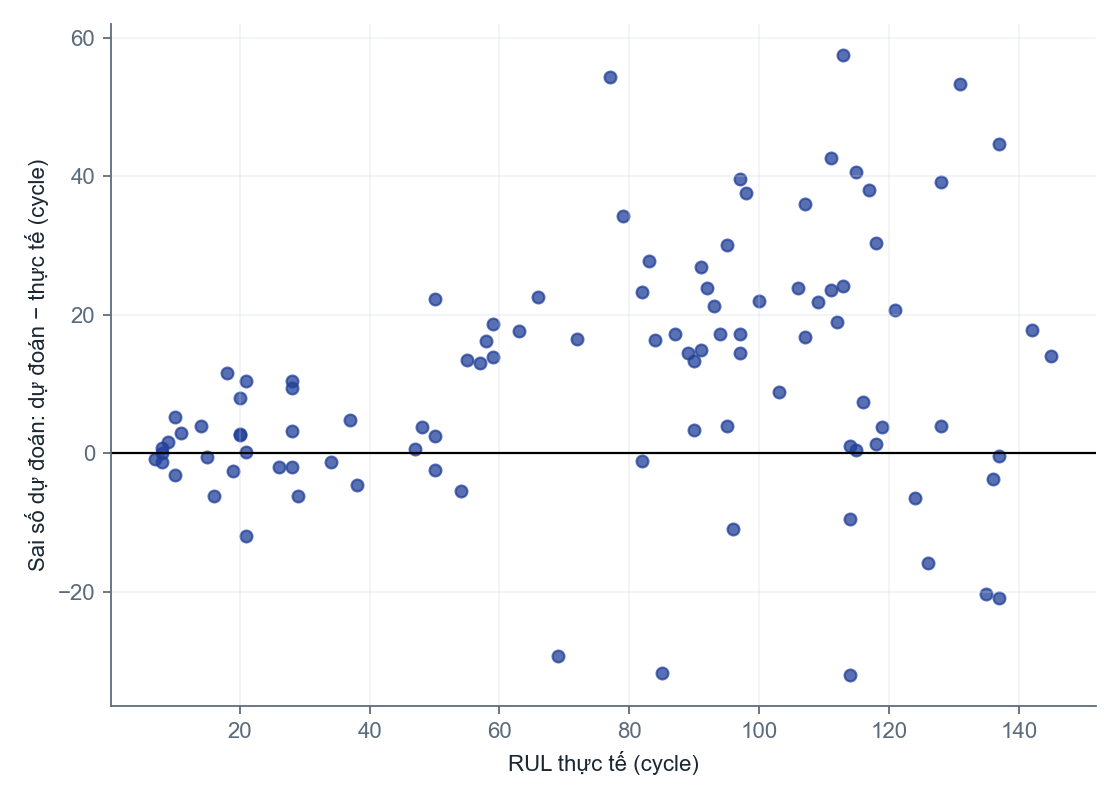
\includegraphics[width=\textwidth]{../outputs/modeling/figures/final_residuals_by_rul.png}
\column{0.40\textwidth}
74 dự đoán cao hơn RUL thật; 26 dự đoán thấp hơn.

\vspace{0.45cm}
\begin{block}{Trường hợp sai lớn}
Engine 23: RUL thật 113; dự đoán 170,4768; absolute error 57,4768 cycles.
\end{block}

Metric trung bình không thay thế việc xem các failure case.
\end{columns}
\source{outputs/modeling/figures/final_residuals_by_rul.png}
\end{frame}

\begin{frame}{Phân tích phụ: Health Index và ARIMA}
\begin{columns}[T,onlytextwidth]
\column{0.55\textwidth}
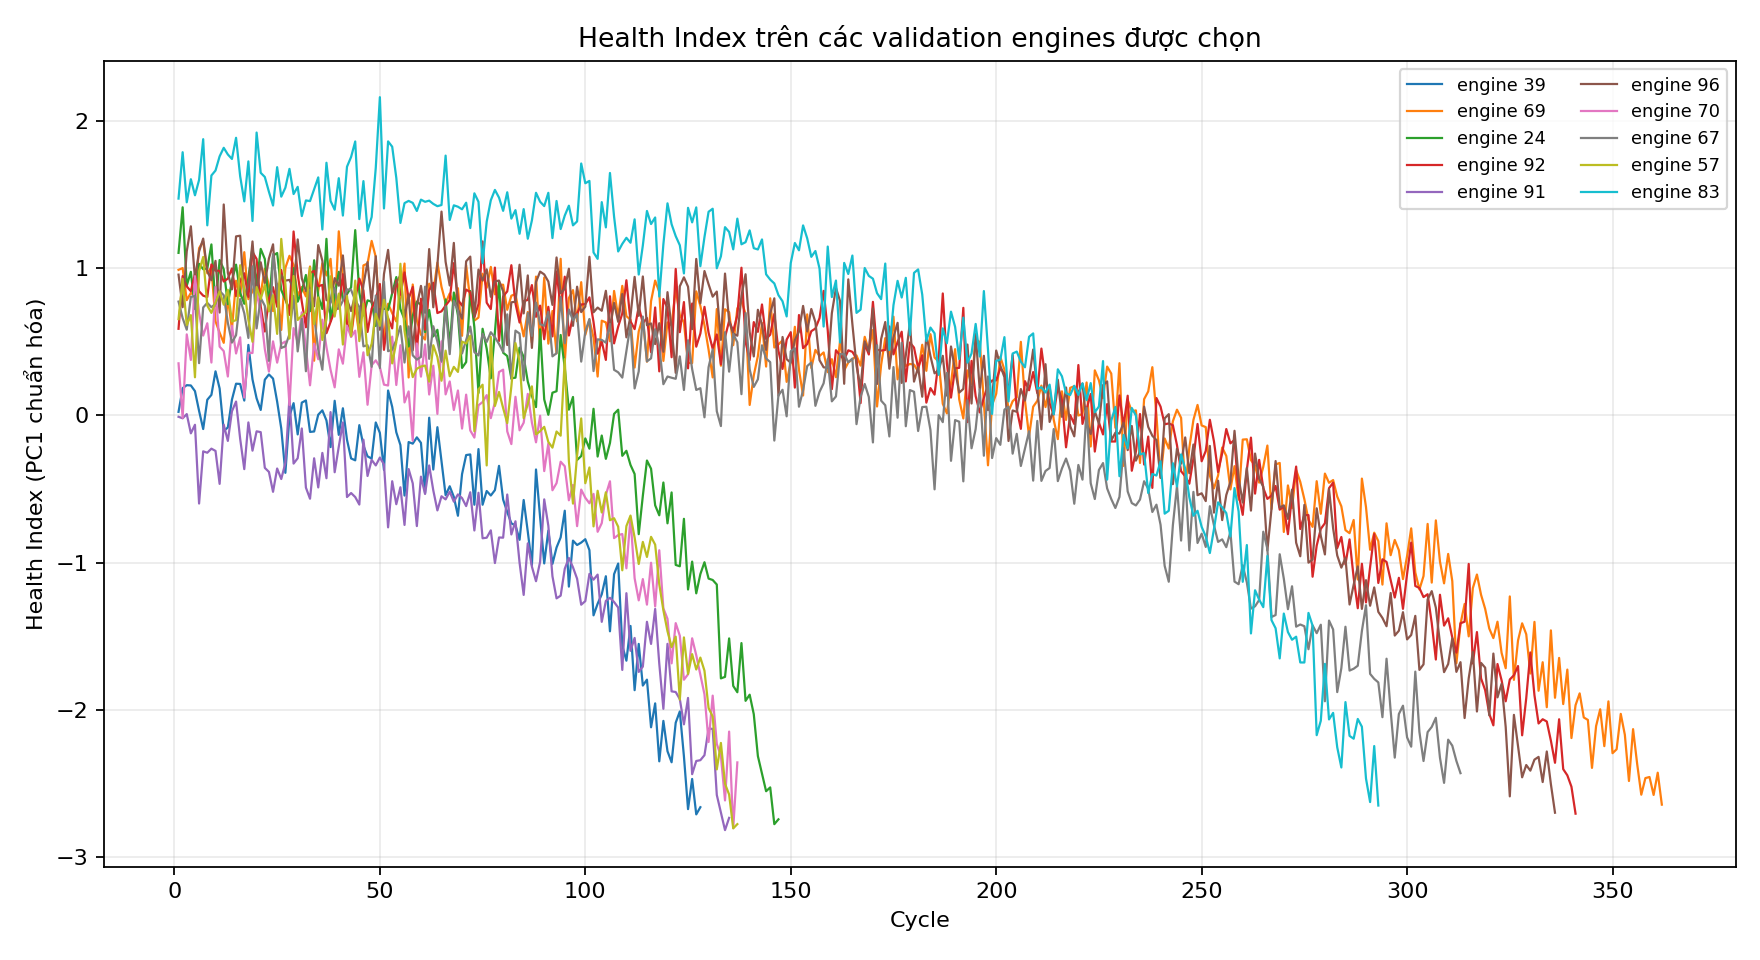
\includegraphics[width=\textwidth]{../outputs/timeseries/figures/health_index_selected_engines.png}
\column{0.41\textwidth}
\begin{table}
\centering\scriptsize
\begin{tabular}{lrr}
\toprule
Dự báo & MAE & RMSE\\
\midrule
ARIMA & 0,4110 & 0,5027\\
Drift & 0,7469 & 0,9128\\
Last-value & 0,9478 & 1,1553\\
\bottomrule
\end{tabular}
\end{table}

ARIMA forecast Health Index, không phải RUL. Coverage prediction interval thay đổi
từ 21,43\% đến 97,03\%.
\end{columns}
\source{outputs/timeseries/tables/baseline_metrics.csv; outputs/timeseries/tables/forecast_metrics.csv}
\end{frame}

\begin{frame}{Cảnh báo sớm từ RUL dự đoán}
Ngưỡng cảnh báo cố định: $\mathrm{RUL}\leq30$ cycles trên selected-model OOF train.

\begin{table}
\centering
\begin{tabular}{lr}
\toprule
Timing & Số engine\\
\midrule
Trước ngưỡng & 44\\
Đúng ngưỡng & 7\\
Sau ngưỡng nhưng trước failure & 49\\
\bottomrule
\end{tabular}
\end{table}

Lead time có trung vị 30 cycles, miền 19--55 cycles. OOF đã dùng để chọn model,
nên đây là mô tả nội bộ, chưa phải đánh giá độc lập về utility bảo trì.
\source{outputs/modeling/tables/warning_summary.json}
\end{frame}

\begin{frame}{ETL và khả năng tái lập}
\begin{block}{Parity ETL}
Pandas và PySpark khớp tại ba boundary Silver/Gold; sai khác tuyệt đối lớn nhất bằng 0.
\end{block}

\begin{block}{Benchmark}
Benchmark runtime chỉ đo Pandas in-memory trên dữ liệu nhân bản; chưa phải benchmark cluster.
\end{block}

\begin{block}{Kiểm chứng}
Full test suite hiện tại đạt 175 tests. Artifact lưu config, raw hash, metric và provenance.
\end{block}
\source{outputs/etl/parity.json; outputs/etl/benchmark.json}
\end{frame}


\begin{frame}{Thiết kế thử nghiệm cải thiện RUL}
\begin{block}{Phạm vi đã chạy}
Window 10/20/30, 24 cấu hình HGB và ba phương án trọng số RUL.
Các phương án dùng cùng 17.731 khóa từ cycle 30 của 100 train engines.
\end{block}
\begin{block}{Tách lựa chọn và đánh giá}
5 outer folds theo engine. Mỗi outer train dùng inner 3-fold chọn cấu hình,
sau đó mới đánh giá trên outer validation.
\end{block}
\begin{block}{Tiêu chí}
Ưu tiên MAE khi RUL $\leq30$. MAE toàn bộ, tỷ lệ cảnh báo trễ và thời gian
báo sớm phải không tăng so với baseline của giai đoạn.
\end{block}
\source{experiments/README.md; 20260927_full/search_manifest.json}
\end{frame}

\begin{frame}{Kết quả chưa đạt tiêu chí cải thiện}
\small
Outer evaluation trên cùng 100 train engines, từ cycle 30.
\begin{table}
\centering\small
\begin{tabular}{lrrr}
\toprule
Phương án & MAE toàn bộ & MAE RUL $\leq30$ & Trễ/bỏ lỡ\\
\midrule
Baseline & 20,2143 & 3,6676 & 49/100\\
Sau chọn window & 20,2143 & 3,6676 & 49/100\\
Sau chỉnh tham số & 20,2459 & 3,6730 & 53/100\\
Sau chọn trọng số & 20,2459 & 3,6730 & 53/100\\
\bottomrule
\end{tabular}
\end{table}
MAE RUL thấp thay đổi $+0{,}0054$ cycles, CI 95\%
$[-0{,}0506;0{,}0639]$. Cảnh báo trễ tăng 4 điểm phần trăm, CI $[1;8]$.
\begin{block}{Cấu hình cuối}
Chọn lại baseline. Test MAE vẫn là 15,3490 cycles trên 100 engines.
\end{block}
\source{20260927_full/ablation_metrics.csv; paired_comparison.csv}
\end{frame}

\begin{frame}{Giảm sai số có thể đi kèm đánh đổi}
\small
Ví dụ trong inner CV trên toàn train, phục vụ chọn cấu hình.
\begin{table}
\centering\small
\begin{tabular}{lrrr}
\toprule
Ứng viên & MAE RUL $\leq30$ & MAE toàn bộ & Trễ/bỏ lỡ\\
\midrule
Baseline & 3,6148 & 20,3613 & 50/100\\
\texttt{hgb\_08} & 3,2625 & 20,6846 & 49/100\\
Ưu tiên RUL thấp cao & 3,3901 & 20,4072 & 47/100\\
\bottomrule
\end{tabular}
\end{table}
\texttt{hgb\_08} giảm MAE RUL thấp khoảng 9,75\% nhưng tăng MAE toàn bộ
0,3233 cycles. Phương án trọng số cao còn tăng tỷ lệ thời gian báo sớm.
\begin{block}{Diễn giải}
Chưa thay model theo tiêu chí đã chốt. Đợt tiếp theo cần công bố mức đánh đổi
chấp nhận được trước khi thử lại. Bảng này chưa phải đánh giá ngoài độc lập.
\end{block}
\source{20260927_full/final_selection_metrics.csv}
\end{frame}

\begin{frame}{Kết luận và giới hạn}
\begin{block}{Kết quả chính}
HistGradientBoosting đạt MAE 15,3490 cycles trên FD001 với window 30.
\end{block}

\begin{block}{Giới hạn}
FD001 là dữ liệu mô phỏng; test đánh giá một điểm cắt mỗi engine; đợt nested CV mới chưa đạt tiêu chí cải thiện; không có cost, downtime hoặc intervention records.
\end{block}

\begin{block}{Bước tiếp theo}
Chốt mức đánh đổi cho vùng RUL thấp, thử đặc trưng mới trong training fold và công bố protocol trước đợt tiếp theo.
\end{block}
\source{report/sections/conclusion.tex; outputs/cross_dataset/matrix.json}
\end{frame}

\begin{frame}{Transfer giữa các subset C-MAPSS}
\small
Ma trận bổ sung dùng window 10 cycles vì test FD004 có engine ngắn nhất 19 cycles.

\begin{table}
\centering\scriptsize
\begin{tabular}{llrr}
\toprule
Train $\rightarrow$ Test & Loại & MAE & RMSE\\
\midrule
FD001 $\rightarrow$ FD001 & Nội bộ & 21,9258 & 29,5936\\
FD002 $\rightarrow$ FD002 & Nội bộ & 22,3556 & 31,3077\\
FD003 $\rightarrow$ FD003 & Nội bộ & 28,3255 & 41,7606\\
FD004 $\rightarrow$ FD004 & Nội bộ & 27,2218 & 36,9311\\
FD001 $\rightarrow$ FD002 & Transfer & 60,3215 & 70,4603\\
FD001 $\rightarrow$ FD003 & Transfer & 47,3949 & 59,2140\\
FD001 $\rightarrow$ FD004 & Transfer & 58,5731 & 69,8148\\
\bottomrule
\end{tabular}
\end{table}

Model fit trên FD001 không nên dùng trực tiếp cho subset khác nếu chưa retraining
hoặc domain adaptation. Metric chính FD001 trên các slide trước dùng window 30,
nên không so trực tiếp với ma trận window 10.
\source{outputs/cross_dataset/matrix.json; outputs/cross_dataset/README.md}
\end{frame}

\end{document}
